\documentclass[table]{beamer}

\mode<presentation>
{
  \useoutertheme{infolines}
  \setbeamercovered{transparent}
  \setbeamertemplate{headline}{\insertnavigation{\textwidth}}
  \setbeamertemplate{footline}[miniframes theme]
%  \setbeamertemplate{frametitle}{\insertlogo \hspace{.1cm} \insertframetitle}
  \setbeamertemplate{navigation symbols}{}
}

\PassOptionsToPackage{table}{xcolor}
\usepackage{xcolor}
\usepackage{graphicx}
\usepackage{xspace}
\usepackage{upgreek}
\usepackage{minted}

\newenvironment{itemize*}%
  {\begin{itemize}%
    \setlength{\itemsep}{.5cm}%
    \setlength{\parskip}{0pt}}%
  {\end{itemize}}
\newenvironment{enumerate*}%
  {\begin{enumerate}%
    \setlength{\itemsep}{.5cm}%
    \setlength{\parskip}{0pt}}%
  {\end{enumerate}}
\newenvironment{append}%
  {\appendix \newcounter{lastframe} \setcounter{lastframe}{\value{framenumber}}}%
  {\setcounter{framenumber}{\value{lastframe}}}

  \title{MC generators}
  \subtitle{status \& plans}
\author[Redmer, jkl]{Redmer Bertens\inst{1}, Jochen Klein\inst{2}}
\institute[]{
  \inst{1} University of Tennessee, Knoxville \and
  \inst{2} CERN, Geneva
}
\date[PAG-MC, Mar 1, 2017]{
  PAG-MC meeting\\[.2cm]
  March 1st, 2017
}
\titlegraphic{
  
\includegraphics[height=1.2cm]{../fig/CERN_logo}\hspace{0.5cm}
  
\includegraphics[height=1.2cm]{../fig/2011-Nov-24-ALICE_logo_WithoutStrapline}\hspace{0.5cm}
}

\newcommand{\pp}{pp}
\newcommand{\ppb}{p--Pb}
\newcommand{\pbpb}{Pb--Pb}
\newcommand{\daq}{DAQ}
\newcommand{\ctp}{CTP}
\newcommand{\pt}{\ensuremath{p_\perp}\xspace}
\newcommand{\gevc}{\ensuremath{\mathrm{GeV}/c}\xspace}
\newcommand{\nsp}{\ensuremath{N_{\sigma, \text{p}}}\xspace}
\newcommand{\cred}[1]{\relax {\small \textcolor{blue!70}{[#1]}}}
\newcommand{\concl}[1]{\textcolor{gray}{\hrule}\begin{center}#1\end{center}}

\begin{document}

{
  \setbeamertemplate{footline}{}
  \setbeamertemplate{headline}{}
  \begin{frame}
    \titlepage
  \end{frame}
}

\begin{frame}{generator validation}
  strategy:
  \begin{itemize}
    \setlength{\itemsep}{.25cm}
  \item use on-the-fly LEGO train:\\
    \href{https://alimonitor.cern.ch/trains/train.jsp?train_id=107}{MM\_MCGen\_validation}
  \item add standard plots for validation:\\[.2cm]
    use existing developments by Christian Bourjau,\\
    see \texttt{\$ALICE\_PHYSICS/PWGMM/MC/aligenqa}
  \end{itemize}
  \vspace{.25cm}
  in progress:
  \begin{itemize}
    \setlength{\itemsep}{.25cm}
  \item setting up of standard generators in progress
  \item QA plots get published on web page\\
    (manually triggered for now)
  \item to be run at each update of generator/configuration
  \item extend set of plots as needed
  \end{itemize}
\end{frame}

\begin{frame}{Anaysis train: MM\_MCGen\_validation}
Generator naming scheme
\begin{itemize}
    \item $[$generator$]\_[$version$]\_[$tune$]\_[$options$]\_[$energy$]$
        \item e.g.Pythia$\_$6$\_$Perugia$\_$noCR$\_$13TeV
\end{itemize}
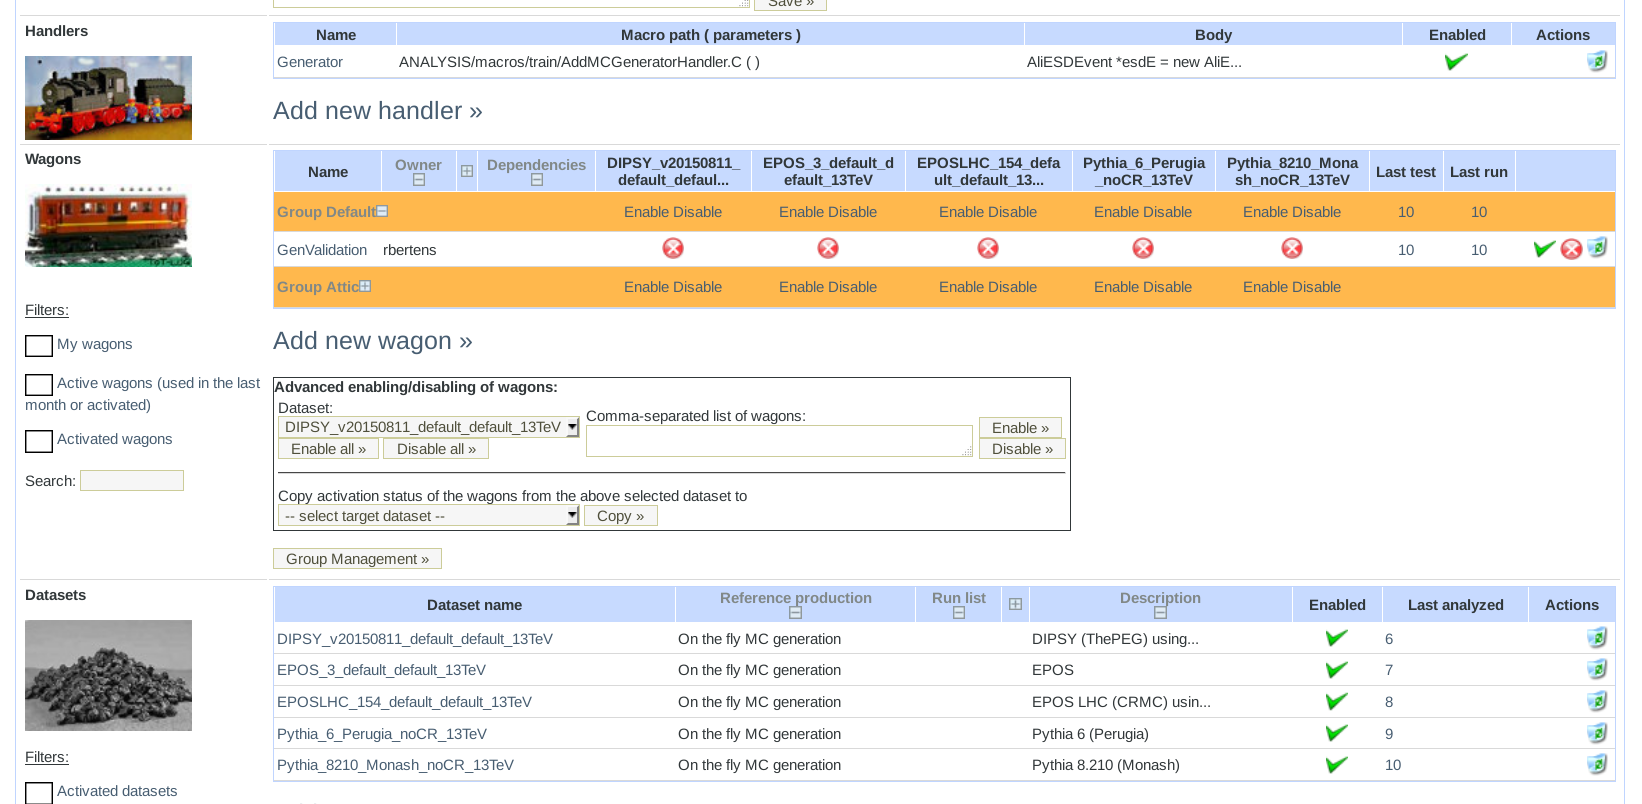
\includegraphics[width=\textwidth]{../fig/pwg_mm_lego_train.png}
\end{frame}


\begin{frame}{Automated QA of generators}
Generator output is analyzed using validation tool
\begin{itemize}
    \item PWG$/$HMTF$/$macros$/$AddTaskHMTFMCMultEst.C
    \item Output published to public webpage
\end{itemize}
    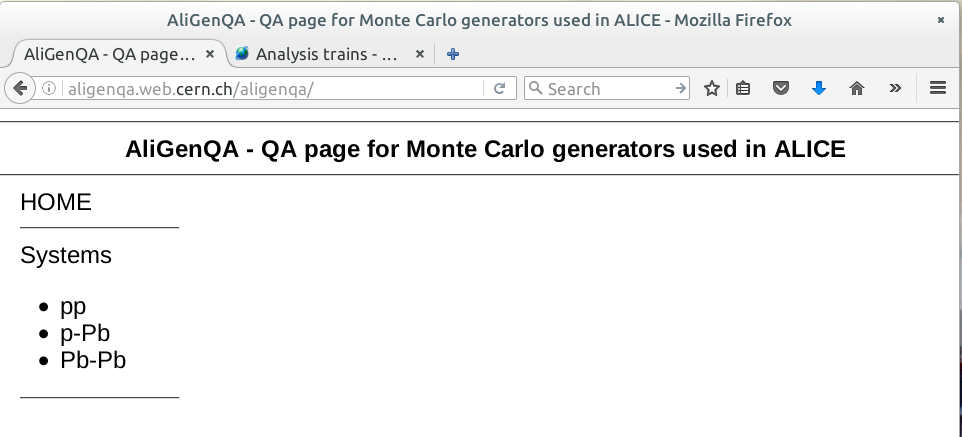
\includegraphics[width=\textwidth]{../fig/aligenqa_webpage.png}
\end{frame}

\begin{frame}{Automated QA of generators}
    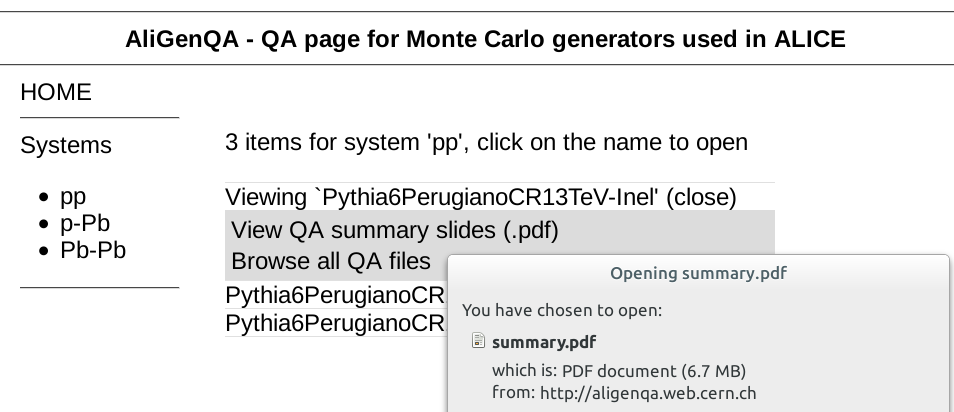
\includegraphics[width=\textwidth]{../fig/open_page.png} \\
    Clicking on a system (pp, p--Pb, Pb--Pb) opens list of generators for which QA is available
\begin{itemize}
    \item Naming scheme analogous to validation train naming scheme, trigger configuration added as suffix
    \item Access to QA summary and to collection of independent figures
\end{itemize}
\end{frame}

\begin{frame}{Automated QA of generators}
    \begin{center}
    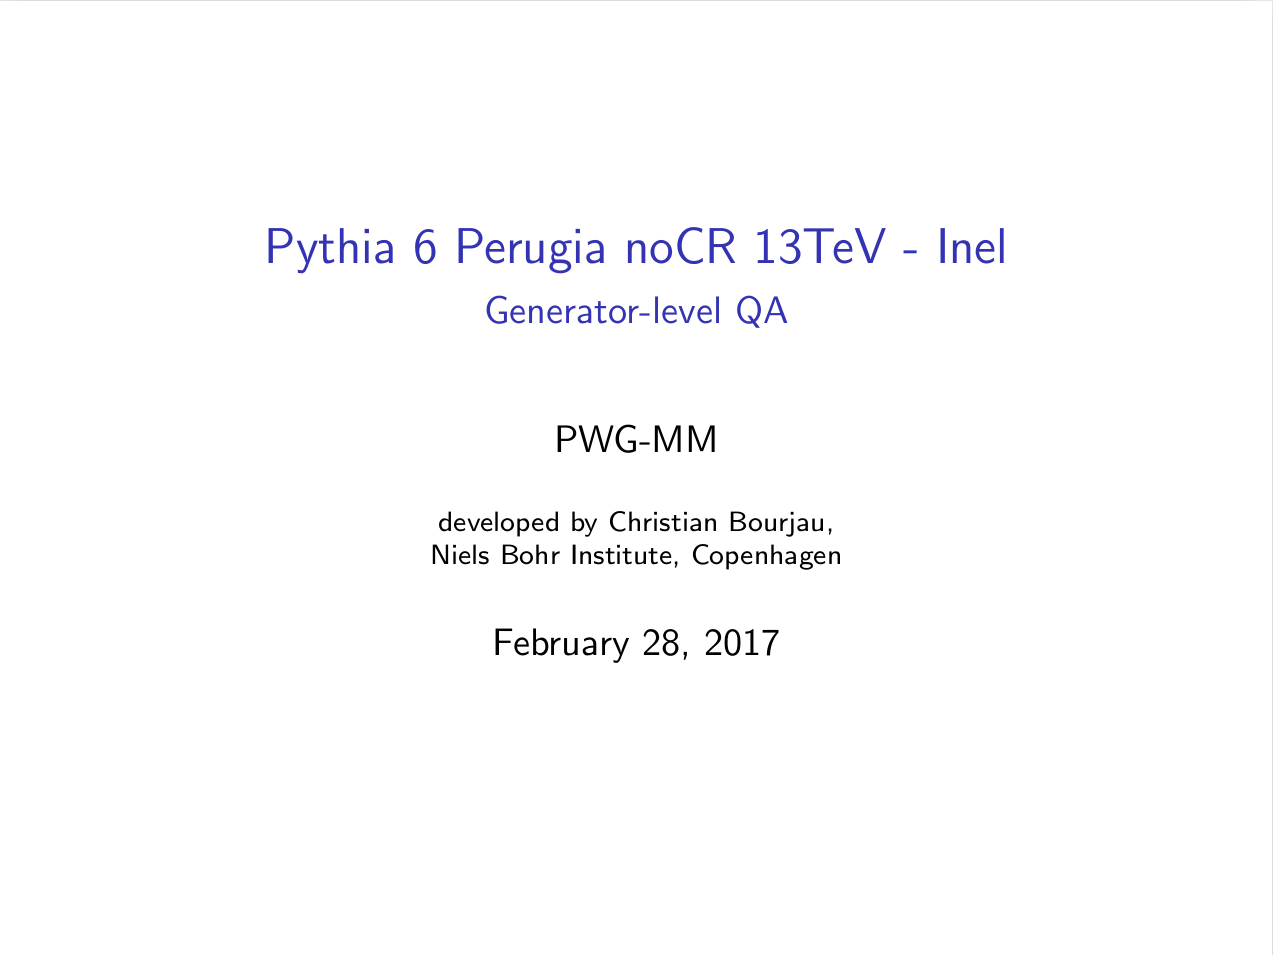
\includegraphics[width=.45\textwidth]{../fig/slide_a.png}
    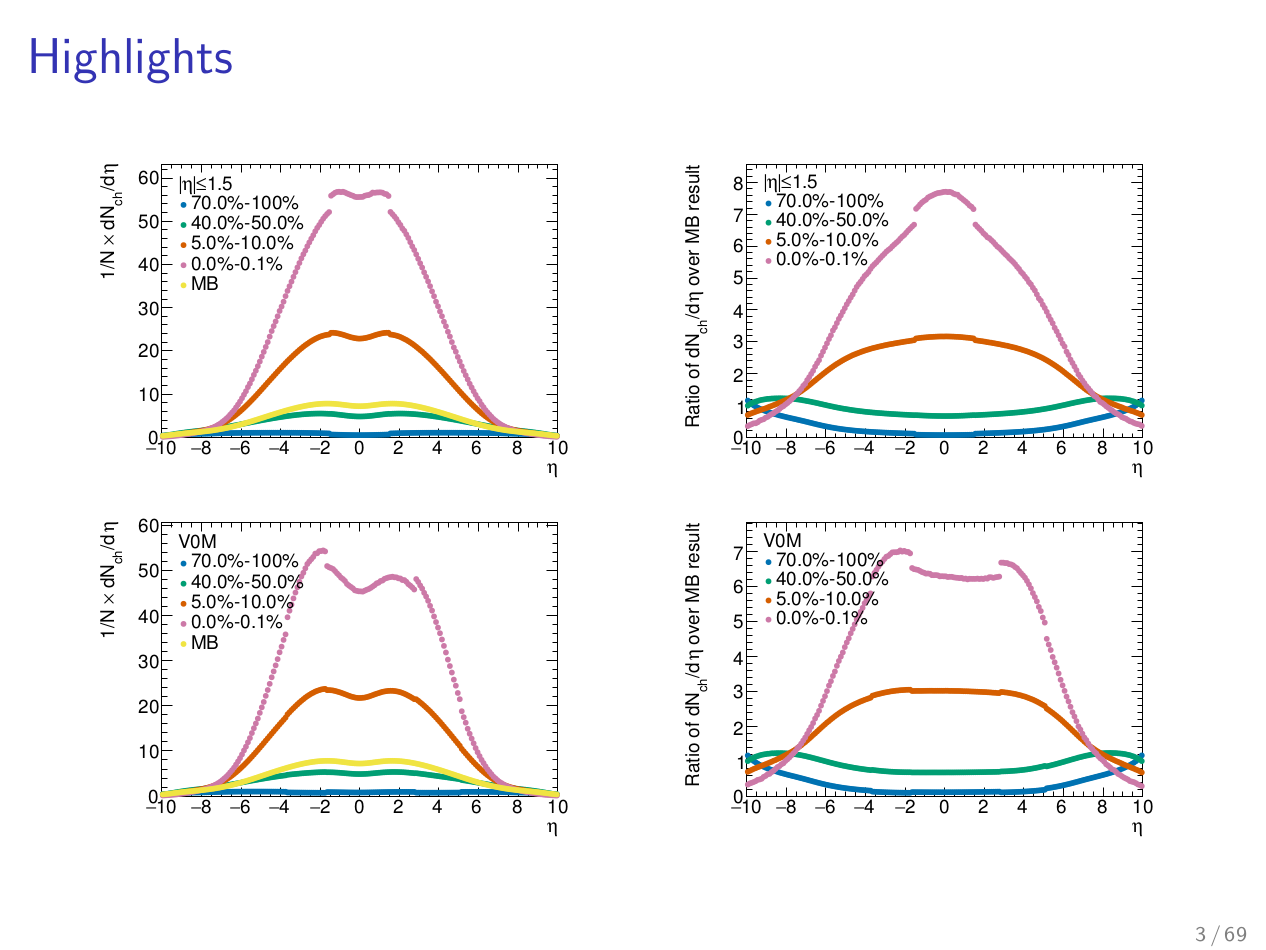
\includegraphics[width=.45\textwidth]{../fig/slide_b.png}\\
    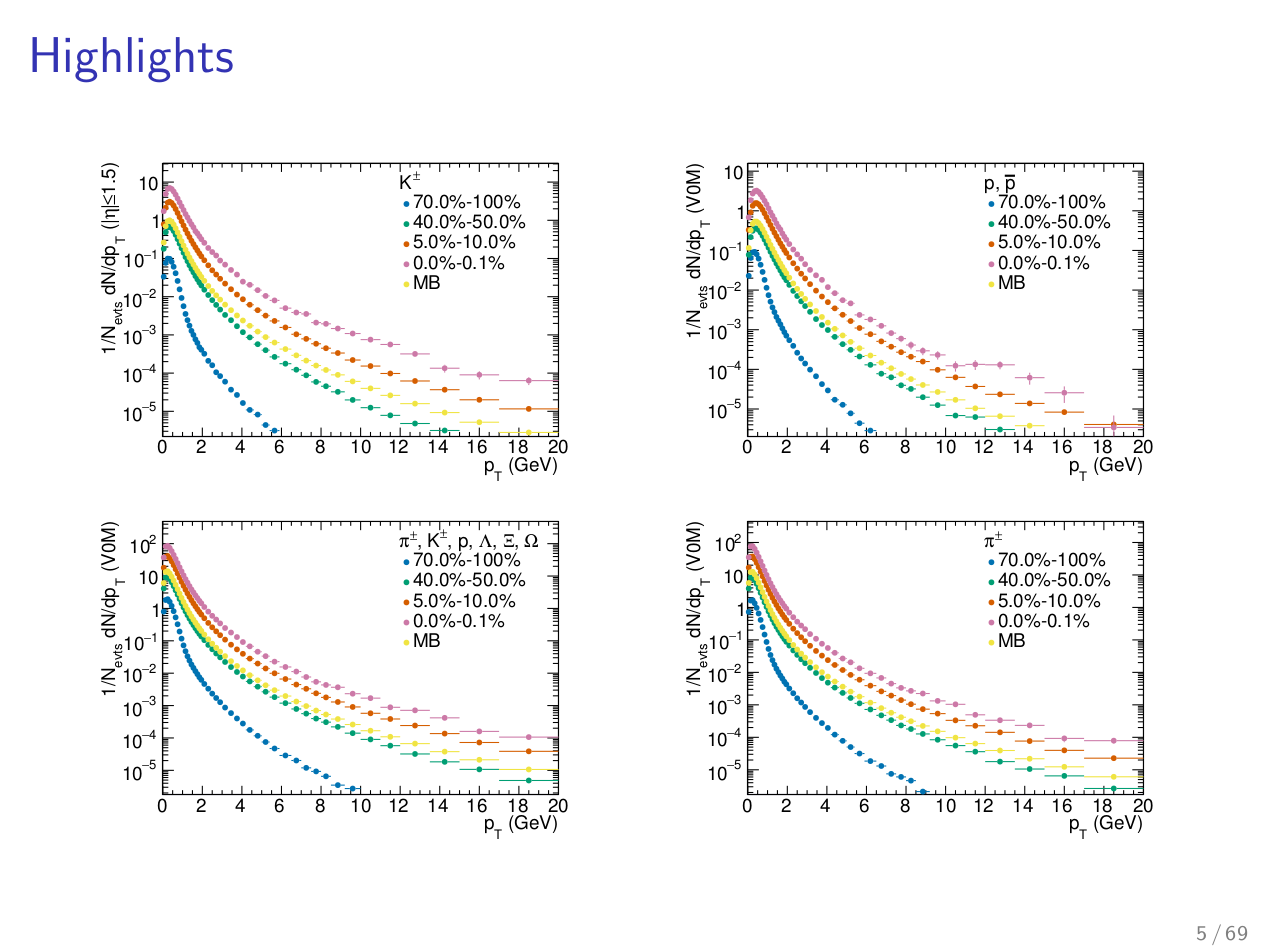
\includegraphics[width=.45\textwidth]{../fig/slide_c.png}
    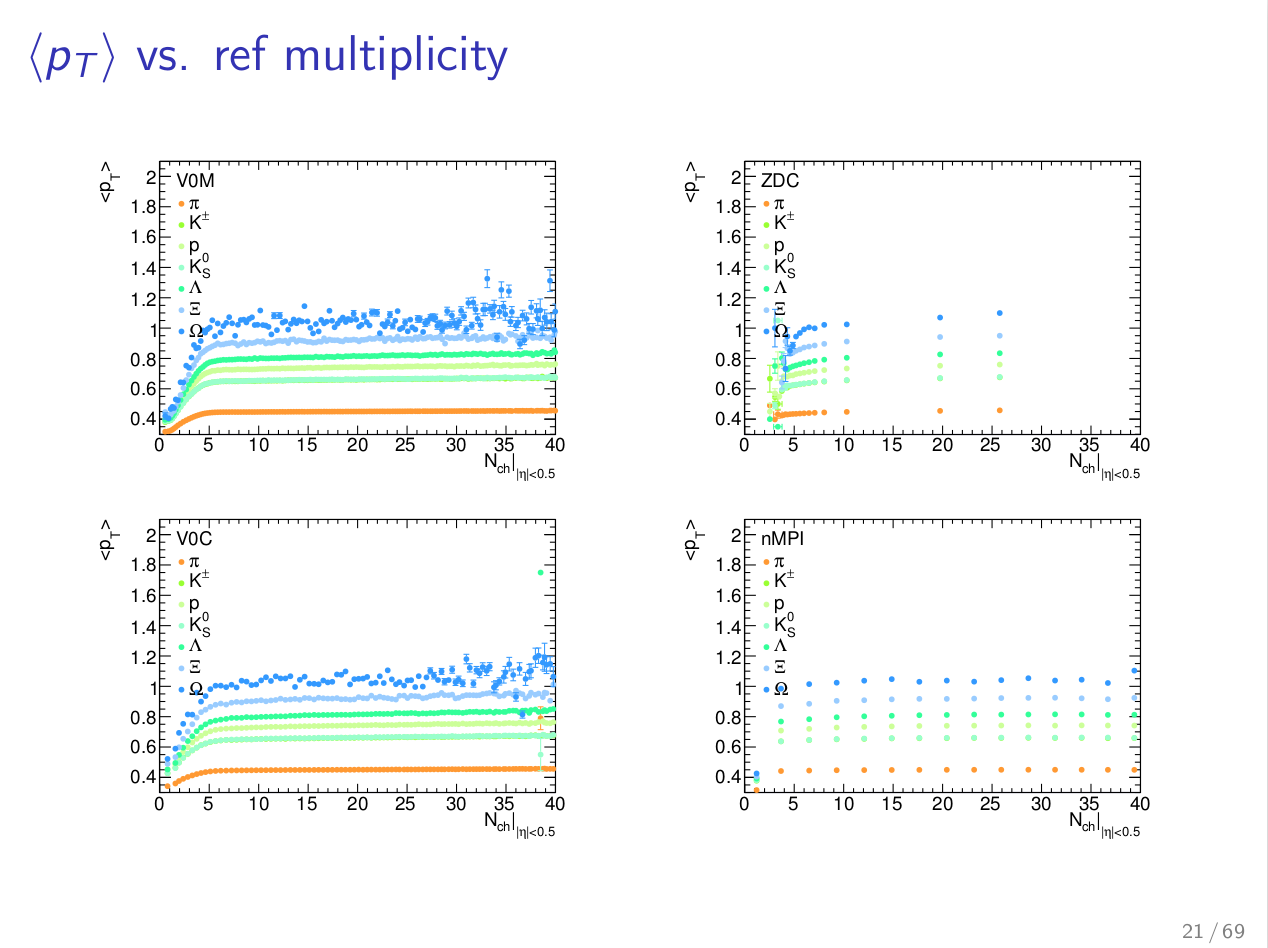
\includegraphics[width=.45\textwidth]{../fig/slide_d.png}
\end{center}
\end{frame}


\begin{frame}{Automated QA of generators}
    Automated QA (for now) organized in
\begin{itemize}
    \item pp
    \item p-Pb
    \item Pb-Pb
\end{itemize}
\vspace{.5cm}

QA figures include
\begin{itemize}
    \item d$N$/d$\eta$, d$N$/d$p_{\text{T}}$ distributions of (un)identified particles
    \item Sets of QA figures for different trigger classes 
    \item Input is welcome!
\end{itemize}
\vspace{.5cm}

TODO:\\
link QA webpage to LEGO train page and production page (for prod QA),\\
to always have full information on generator settings
\end{frame}


\begin{frame}{generators}
  \begin{itemize}
    \setlength{\itemsep}{.25cm}
  \item AMPT
  \item DIPSY
  \item DPMJET
  \item EPOS
  \item EPOS-LHC
  \item Herwig
  \item JEWEL
  \item Pythia 6
  \item Pythia 8
  \item Sherpa
  \end{itemize}
  each with commonly used tunes
\end{frame}

\begin{frame}{generators standalone}
  \begin{itemize}
    \setlength{\itemsep}{.25cm}
  \item provide identical generator setup (incl. tune) as in AliRoot\\
    $\leadsto$ extend wrapper tool \texttt{aligenmc}
  \item make aligenmc available through aliBuild and on cvmfs
  \item also here validation needed:\\
    implement validation as in AliRoot, but using Rivet
  \end{itemize}
\end{frame}

\begin{frame}{Update of AMPT}
  \begin{itemize}
    \setlength{\itemsep}{.25cm}
  \item provide AMPT as stand-alone generator\\
    through aliBuild and on cvmfs
  \item interface to AliRoot, either of:
    \begin{itemize}
    \item dedicated reader in AliRoot
    \item AMPT to HepMC parser
    \end{itemize}
  \item need proper validation of AMPT before doing the update
  \end{itemize}
  will be addressed by Redmer, Alexandru, Jochen
\end{frame}

\begin{append}

  \begin{frame}
    \Huge
    \centering
    Backup
  \end{frame}

\end{append}

\end{document}
